\chapter{Results}
\label{chap:results}

\section{Summary}

Sensitivity testing on benchmark P3HT morphology provided by the Evan and matty work can was finegrained and
used to compare to previous mobility results as well as to test the sensitivity of the algorithm to
reorganization energy, dcut, MSD calculation, and simulation temperature.

On the spot MD simulation of 1000
molecules was performed for testing morph another benchmark OPV material. Janks/mattys work has shown that taking
each monomer to be a chromophore even though charges are known to delocalize on 7 monomers still reproduces
the overall mobility well because the very fast hops along the backbone. I think the application of this
hopping model to ITIC other small molecules is even more justified. Knowing that the this molecule has
negligible electron density in the side chains, chomophores are taking to be the backbone. The effect that
the side chains have on mobility are not a result of electronic contribution to the frontier molecular
orbitals but rather is a result of the effect the chains have on the morphology of the material. 

Delineating chromophores within a morphology needs to be justified by DFT or experiment and balanced against
the computational costs. Furthermore, manually indexing the atoms of the chosen chromophore
remains a significant hurdle. Tutorials on github show how to use the open source tool VMD to speed up this
leg of the workflow. We have also had success with Grits and smarts matching to delineate chromophores through
out the morphology. 

\section{Accuracy}

\begin{table}[ht]
    \caption{Mobility $cm^{2}/Vs$} % title of Table
\centering % used for centering table
\begin{tabular}{c c c c} % centered columns (4 columns)
\hline\hline %inserts double horizontal lines
Software & Amorphous & Semi-crystalline & Crystalline \\ [0.5ex] % inserts table
%heading
\hline % inserts single horizontal line
    ORCA & $0.1085 \pm 0.0006$ & $0.0156 \pm 0.0003$ & $0.123 \pm 0.001$ \\ % inserting body of the table
PySCF & $.0018 \pm .000001$ & $.00148 \pm .000001$ & $.206 \pm 0.0001$ \\ [1ex] % [1ex] adds vertical space
\hline %inserts single line
\end{tabular}
\label{table:nonlin} % is used to refer this table in the text
\end{table}

The results in \ref{table:nonlin} for PySCF were run with a dcut 12. With dcut 10, the crystalline mobility
moves to .15 which is closer to mattys. Waiting on the dcut 10 for the others (semi and disordered). Im very
curious was that will do to their mobilities. All this exploration tells me the workflow is almost two
different things for highly conjugated polyers than it is for amorphous materials. Could a higher dcut in the
semi and amorphous actual make for a slower mobility? I feel like the current numbers are better also. That is
closer to experimentally observed numbers. need more data!!!


\section{Sensitivity}

The sensitivity of the algorithm to various parameter was performed on the benchmark crystalline P3HT
morphology.

\subsection{Neighbor Cutoff (dcut)}

A parameter introduced in the kmc algorithm dcut that trims the fat off of the voronoi neighlist builing.
As can seen from the figure, two points (chromophores) can share cell edges despite being rather far apart. We
therefore, further remove pairs from the neighborlist if they are far enough apart such that it is justifyable
to assume they do not interact electronically enough to effect to charge mobility calc. This parameter will
depend on the material under investigation as was as the size of the individual chromophores. We tested the
sensitivity of the algorithm to the value (dcut). The [zoomed figure] Shows a example dcut radaii. Note that
the z-direction has been collapsed, and the distances do not necessarily correlate to the distance
between chromophores in the system. The figure shows the effect of cutoff distance on value of
16 calculated mobility.


\begin{table}[ht]
\caption{dcut sensitivity}
\centering % used for centering table
\begin{tabular}{c c c c c c c c} % centered columns (4 columns)
\hline\hline %inserts double horizontal lines
dcut & 4 & 6 & 8 & 10 & 12 & 14 & 16 \\ [0.5ex] % inserts table
%heading
\hline  % inserts single horizontal line
pairs & 318 & 22000 & 49000 & 96000 & 113026 & 113315 & 113315 \\ [1ex]% inserting body of the table
$\mu_{0}$ $(cm^{2}/Vs)$ & $-2.17 \cdot 10^{-6}$ & $6.13 \cdot 10^{-4}$ & .01 & .17 & .17 & .22 & .22 \\ [1ex] % [1ex] adds vertical space
%$\mu_{0}$ Error & $-1.75*10^{-6}$ & 6 & 8 & 10 & 12 & 14 & 16 \\
\hline %inserts single line
\end{tabular}
\label{table:dcut-sense} % is used to refer this table in the text
\end{table}

\begin{figure}
  \center
  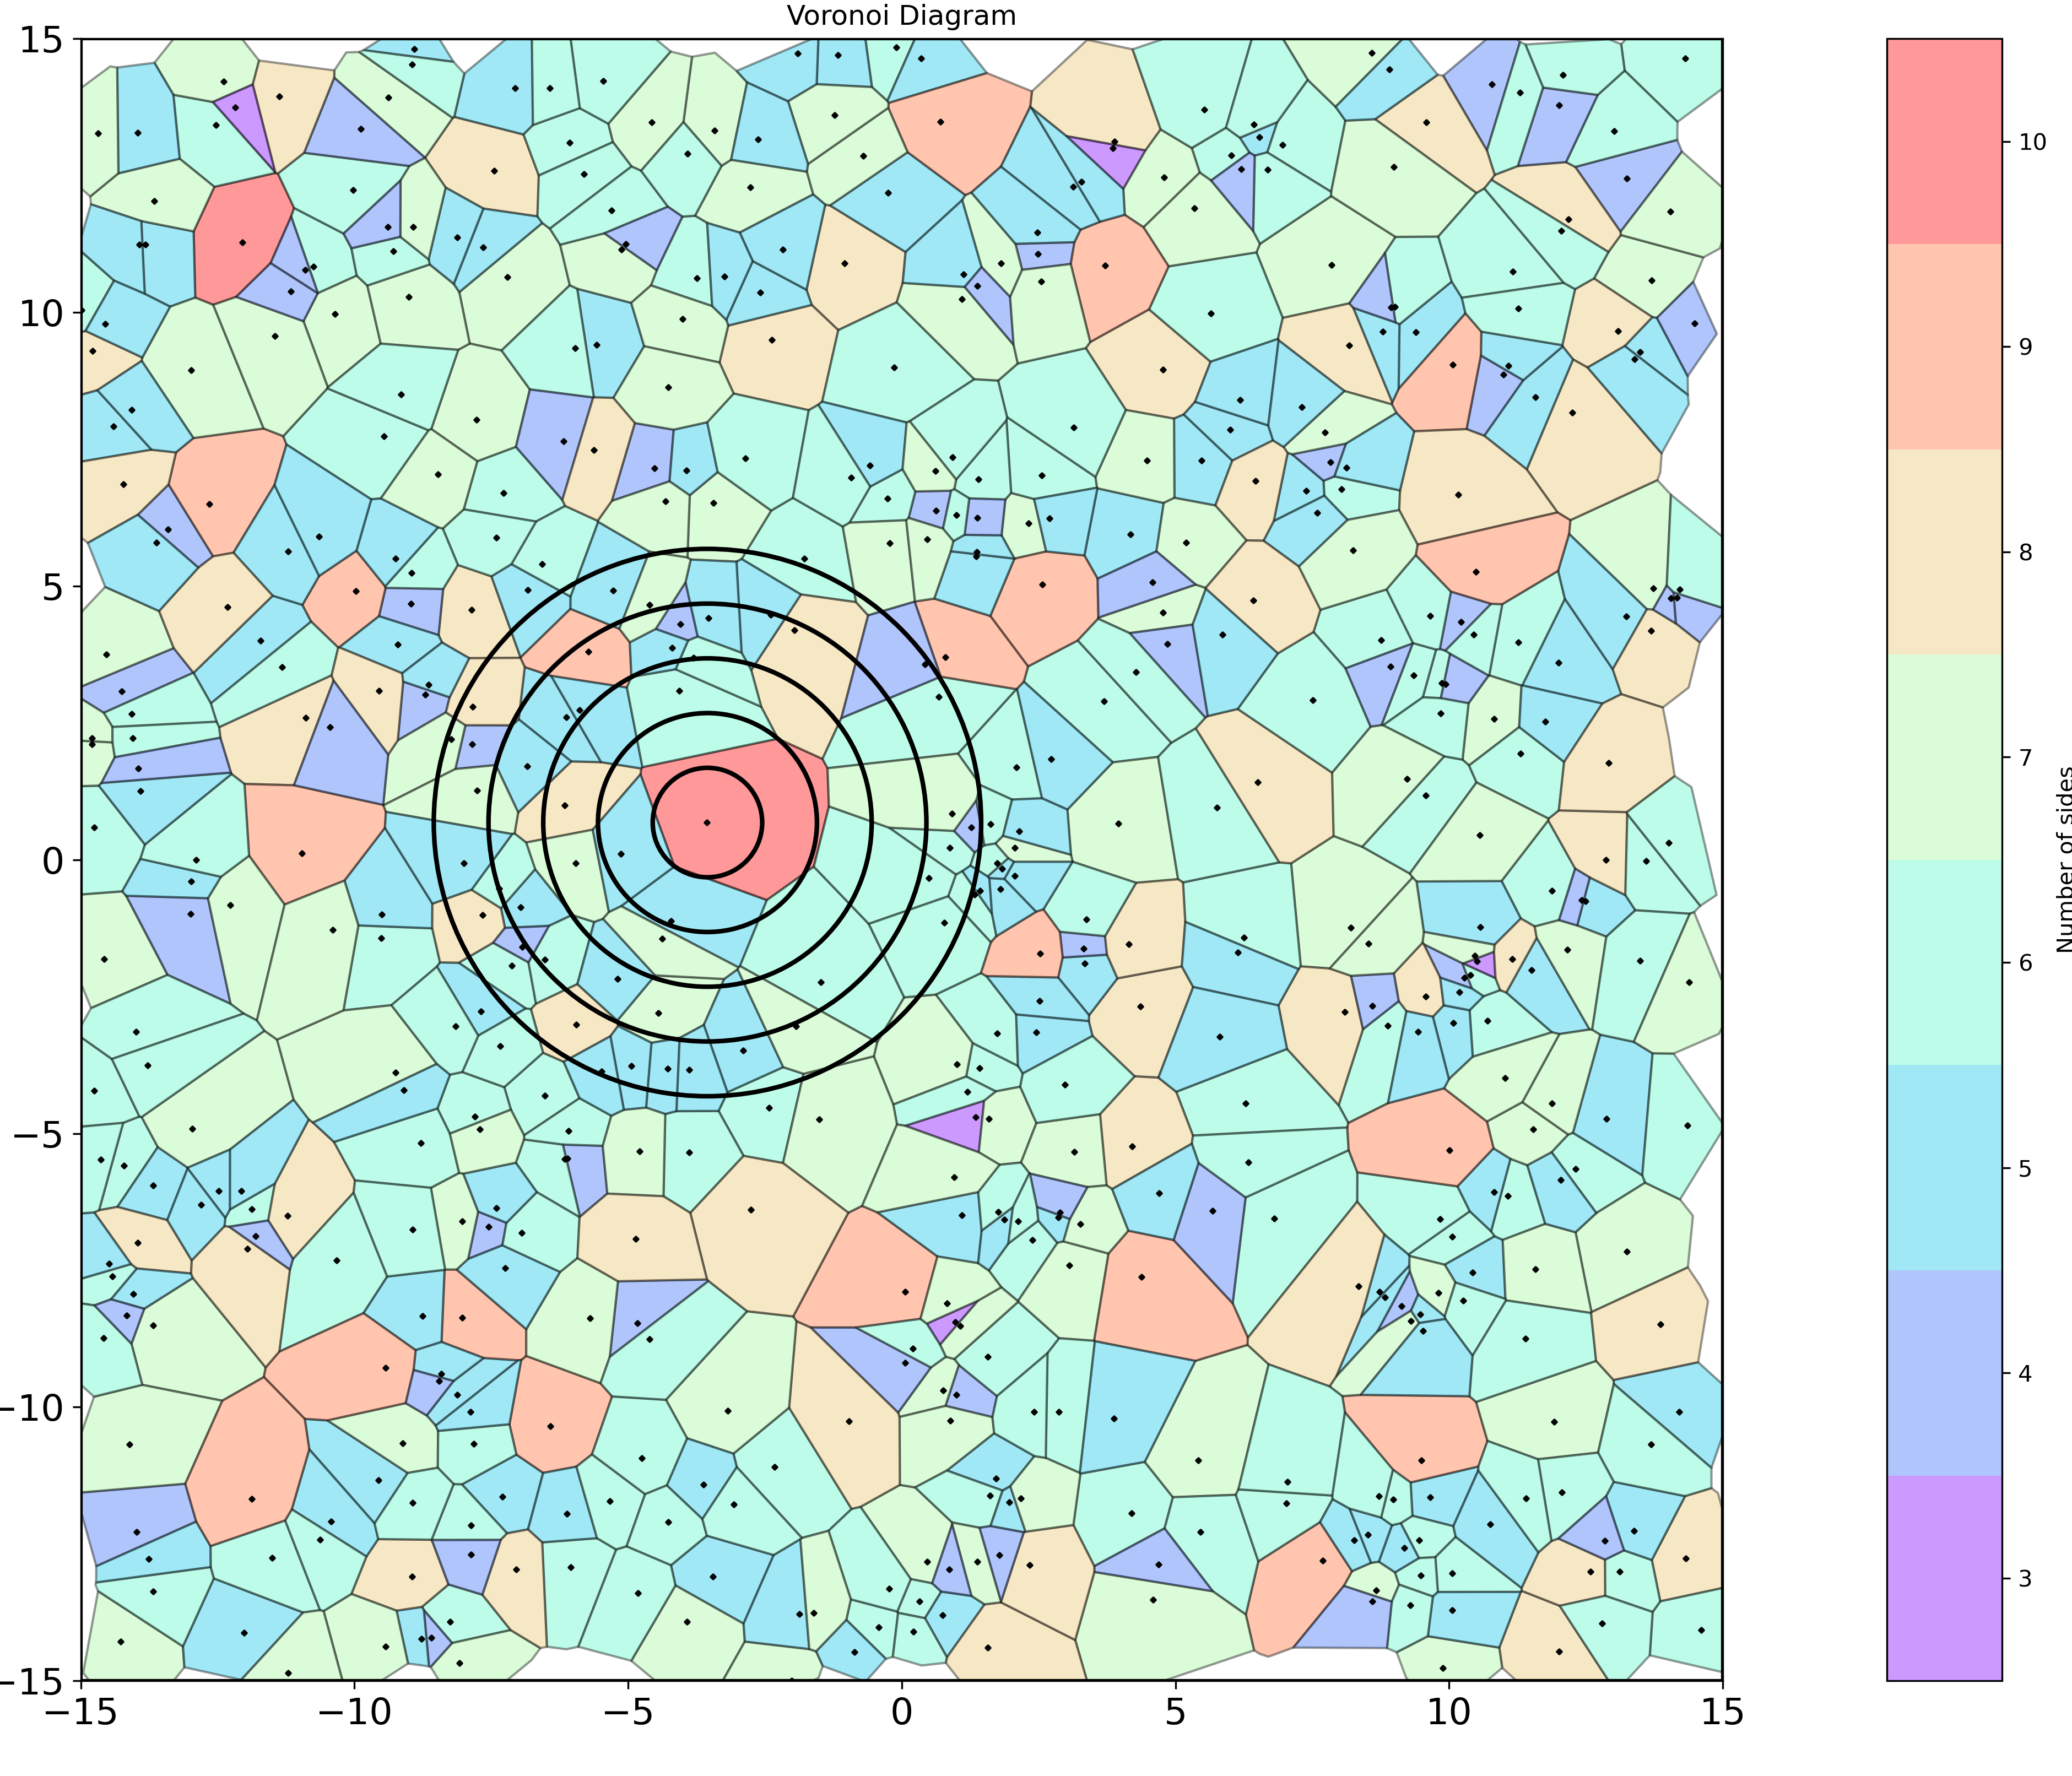
\includegraphics[width=0.8\linewidth]{figures/crystalline_voronoi_d_cut_circles.png} 
  \caption{dcut visual}
  \label{fig:dcut}
\end{figure}


\subsection{Reorganization energy}
Marcus's nonadiabatic electron transfer theory allows us to model charge transfer as two
intersecting parabolic potential energy surfaces. In this work, the parabalas represent the potential energy surface
of the dimer created by a pair of chomophores with a charge injected on either chromophore. In this context, 
reorganization energy, $\lambda_{ij}$, constitutes the energy required to distort the dimer's equilibrium geometry with a
charge on chromophore $i$ into the dimers equillibrium geometry with charge on chromophore $j$.
Reorganization energy consist of the energy change associated with the destortion of the dimers geometry,
and the distortion of the surrounding medium in responce the movement of the charge. It can be written as
follows:
\begin{align}
    \lambda_{total} = \lambda_{internal} + \lambda_{external}.
\end{align} 
$\lambda = 0.3eV$ is chosen to be the default reorganization energy ($\lambda_{internal} = 0.1eV$
and $\lambda_{external} = .02eV$) as others have done with P3HT \cite{jones2017} and
a flourene-triphenylamine copolymer, TFB \cite{Gali2017}. 

\begin{figure}
  \center
  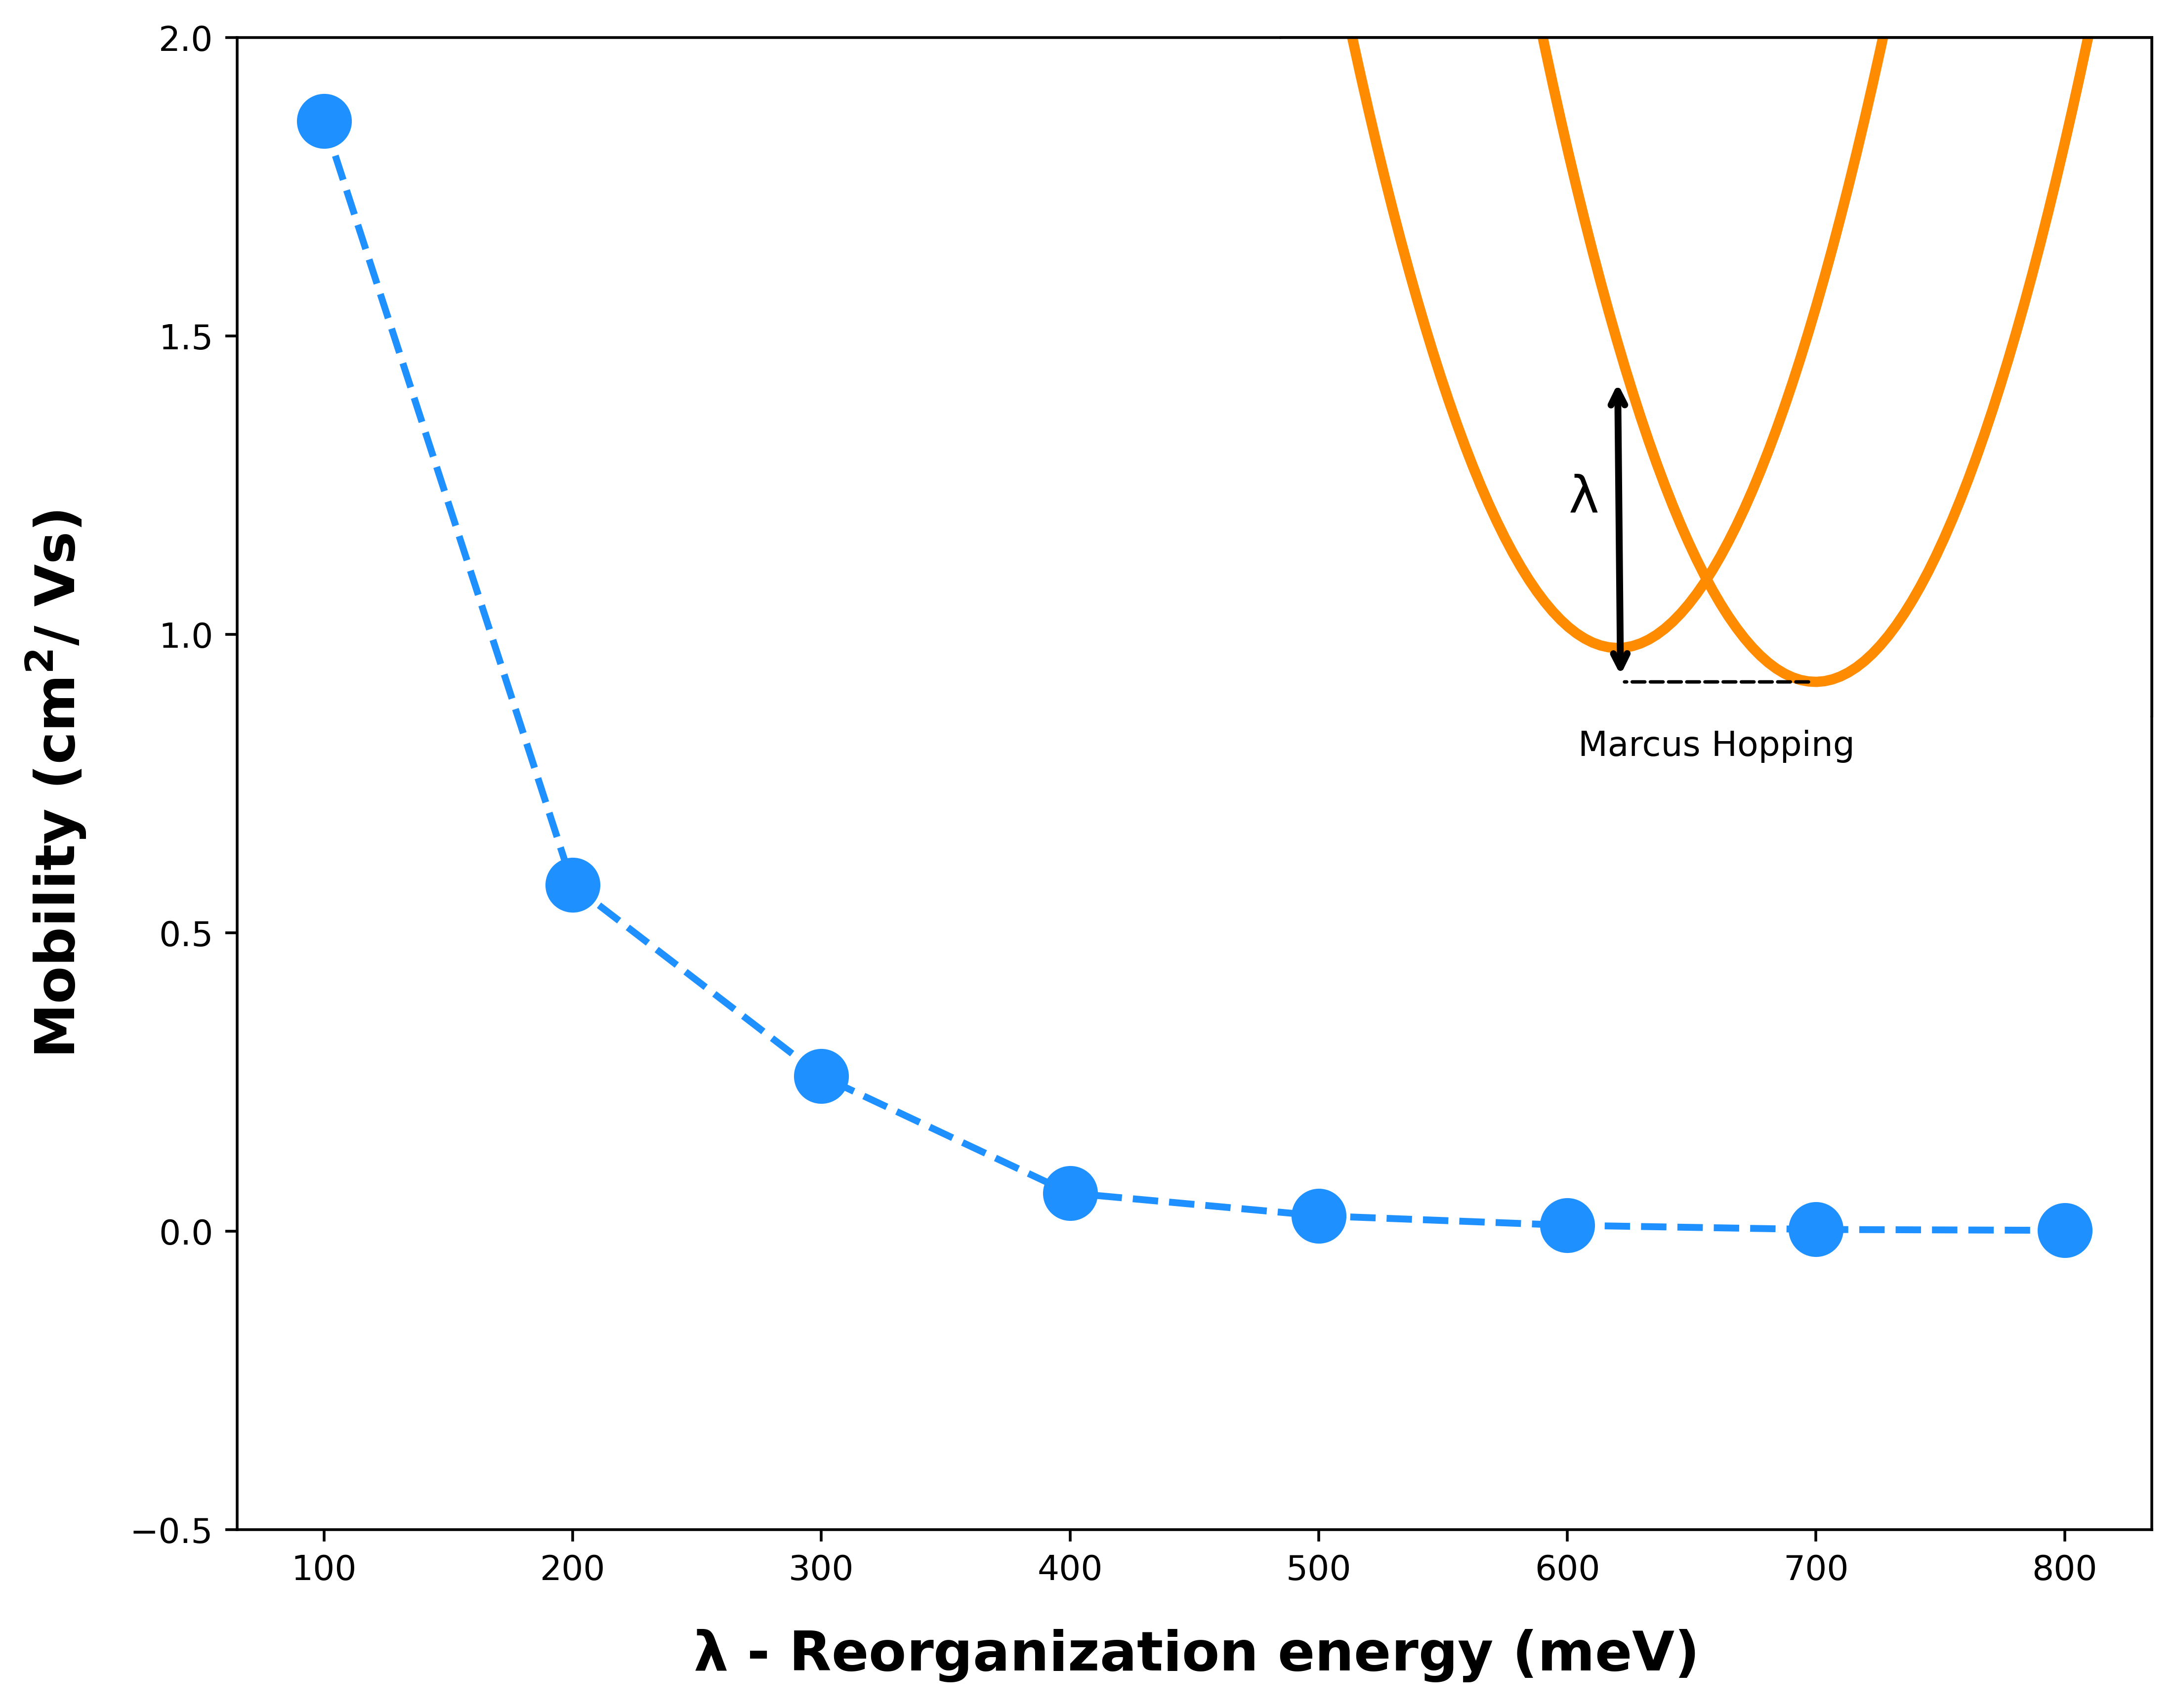
\includegraphics[width=0.8\linewidth]{figures/reorg.png} 
    \caption{The results of running 8 KMC simulations with reorganization energy 100-800 meV}
  \label{fig:reorg}
\end{figure}

\subsection{Temperature}

Another parameter of interest in the Marcus theory mention above is temperuture. To test the sensitivity to
temperature, 15 KMC simulations from 100K to 800k were run on the benchmark P3HT crystalline morphology. It
is clear from the results in [FIGURE] that the mobilities trend upward with temperature. With relatively
weak electronic coupling ($T_{ij}$) between chromophores, electron transfer proceeds nonadiabatically
\cite{clarke2010}. With this weak coupling, the temperature in the Gibbs free energy of activation term
dominates the effect temperature has hop rate. 

\begin{figure}[]
\centering
\begin{subfigure}{.5\textwidth}
    \textbf{(A)}
    \centering
    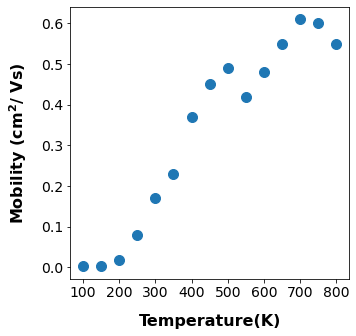
\includegraphics[width=\textwidth]{figures/temp.png}
    \newline
\end{subfigure}%
\begin{subfigure}{.5\textwidth}
    \textbf{(B)}
    \centering
    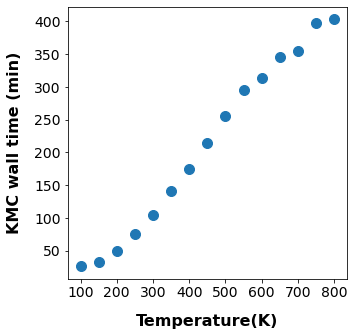
\includegraphics[width=\textwidth]{figures/temp_simtime_plot.png}
    \newline
\end{subfigure}
\begin{subfigure}{.5\textwidth}
    \textbf{(C) 100K}
    \centering
    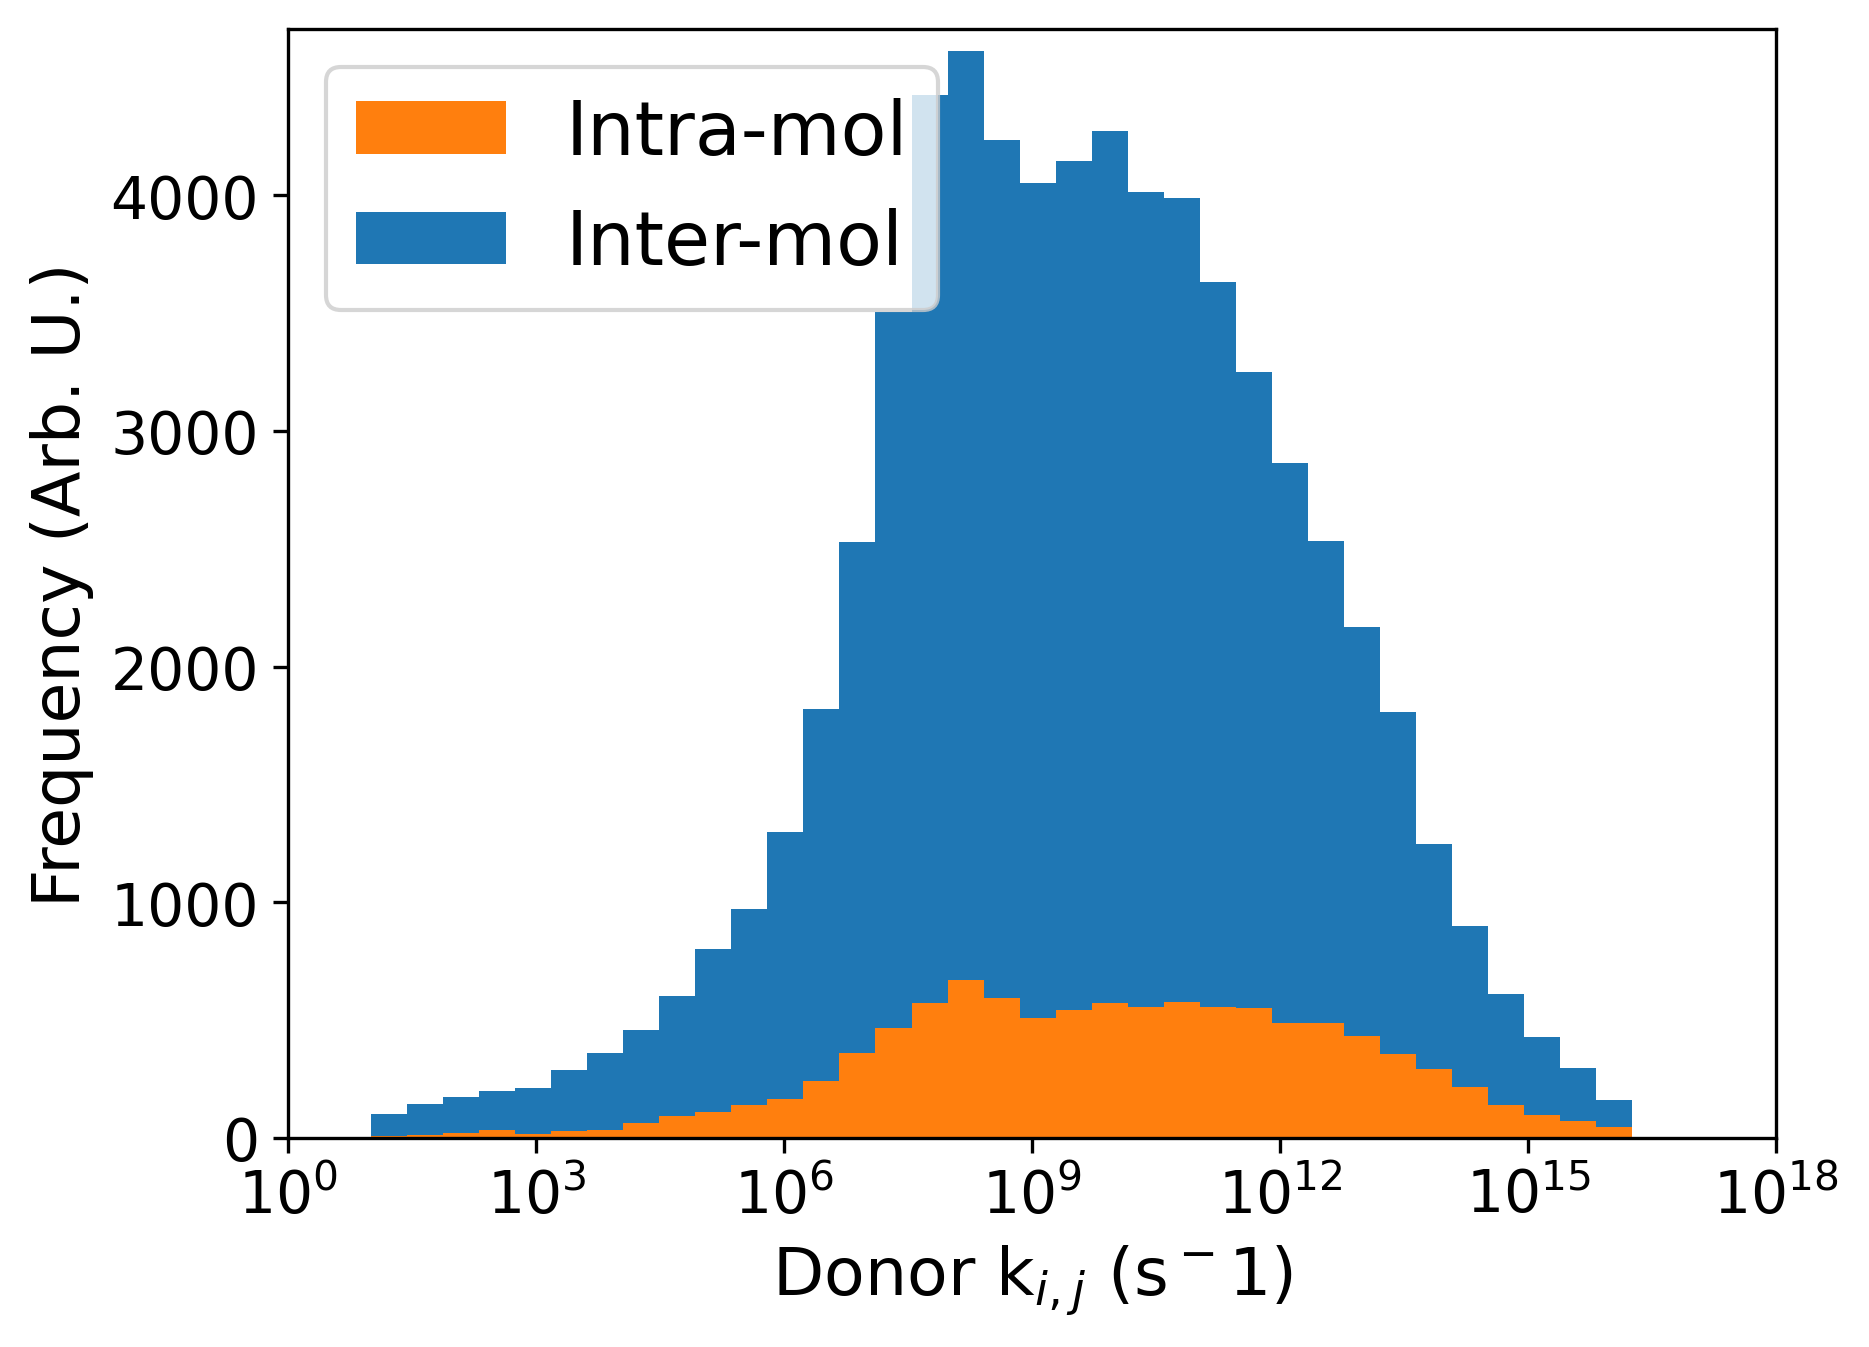
\includegraphics[width=\textwidth]{figures/donor_hopping_rate_clusters_temp100.png}
\end{subfigure}%
\begin{subfigure}{.5\textwidth}
    \textbf{(D) 800K}
    \centering
    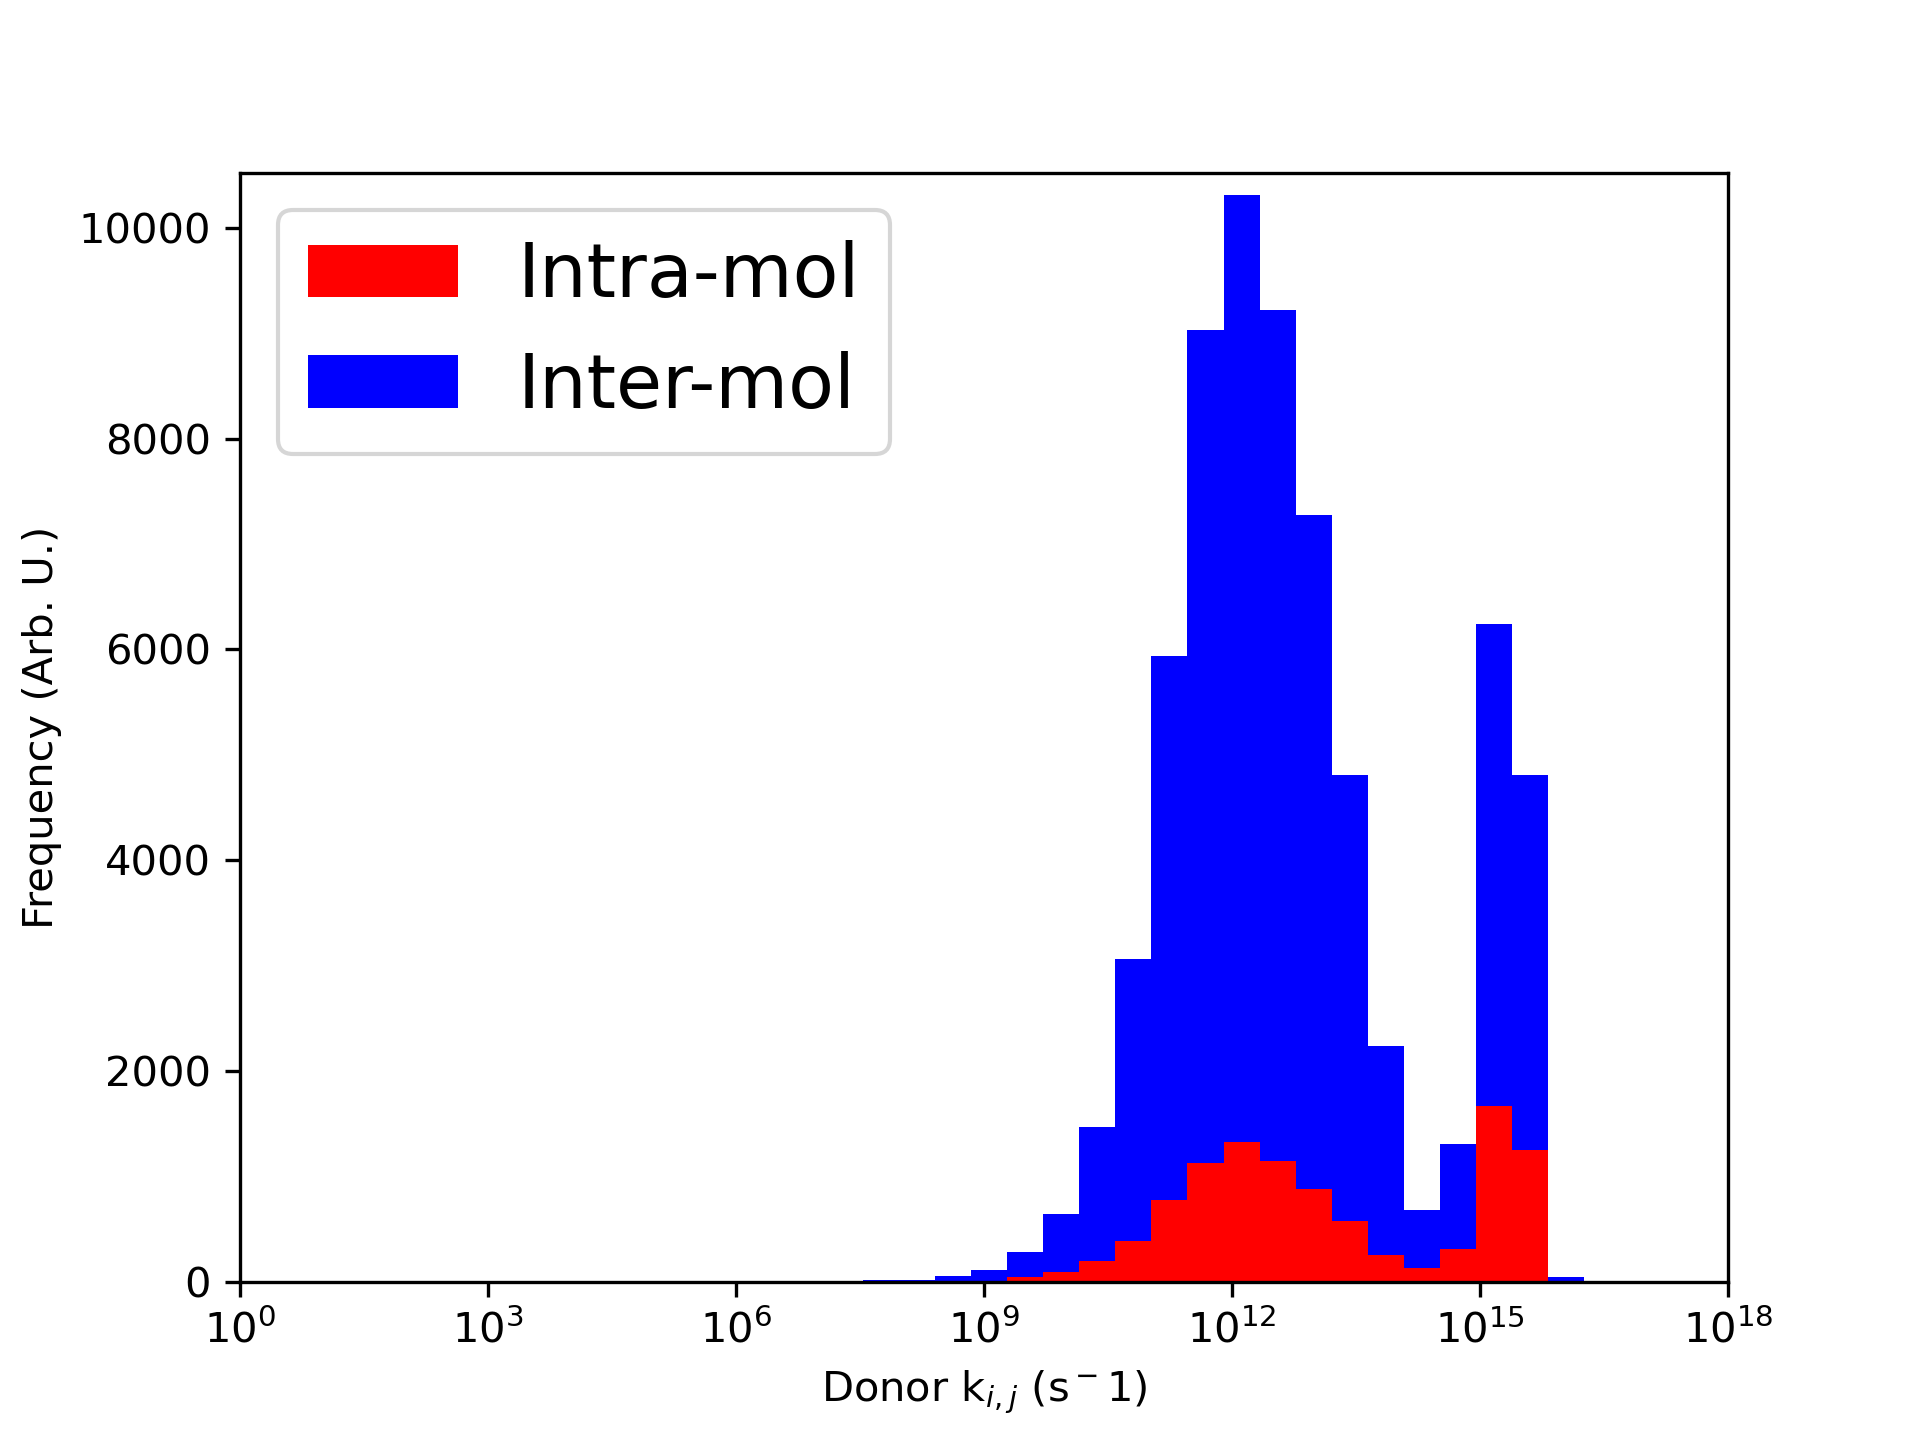
\includegraphics[width=\textwidth]{figures/donor_hopping_rate_clusters_temp800.png}
\end{subfigure}
\caption[short]{A beautiful, well written caption}
\label{TEMP}
\end{figure}

\subsection{MSD (lifetimes)}

The KMC algorithm allows an explicit calculation of the MSD accross a large number of 
particles in the system. Repeating along relevant time scales for 
charge transfer, the slope of this relationship
can be estimated and related to to the 3D diffusion coeffiecient as discussed in the methods section of this
work. Using the Einstien relation (2.3), 
the groundwork for which Einstein derived in his doctoral dissertaion, finally the zero-field
mobility can be obtained. 

It is critical that we not include the ballistic transport timescale in the approximation of the limit
if the slope as time goes to infinity \cite{Maginn2018}. Estimating an upperbound for lifetimes such that
we can estimate the slope of the MSD as time goes to infinity can be messy. In real systems, free chrage
carrier lifetime is subject to a complex interplay between geminate recombination, non-geminate recombination,
charge trapping, temperature, and charge density, whose dynamics play out accros a picosecond to microsecond
timescales and vary widly form material to material as well as from microstrtucture to microstrucute for a
given material \cite{Laquai2015}.

For this work, the primary strategy was to avoid the ballistic region while exploring lifetimes
that are achievable computationally. For example, in an attempt to simulate out to the physical limit, a
simulation a microsecond($10^{-6}s$) lifetime resulted in a single hole hopping for 9 wall time hours.
It is advised that a preanalysis to determine where a given morphology's MSD will convergeb be performed so as
to never simulate past that point. Doing so is superflous and could introduce unessacery noise into the data. 

In the previous work on these P3HT morphologies, 7 liftimes were chosen and a linear regression was performed
to estimate the slope of the MSD. The current work found that the mobility can be apporpriately reproduced
with an appropriate choice of 2 lifetimes beyond the ballistic transport timescale. It was found that with the 
squared displacement averaged over 1000 holes at $10^{-9}s$ and again $10^{-10}s$ the slope of the MSD can be
commensurety reproduced with 1000's less individual holes having to be simulated. The results in the accuracy
section above were aquired with these 2 chosen lifetimes. I am currently running accross 7 lifetimes on the
crystalline morph. 

\begin{figure}
  \center
  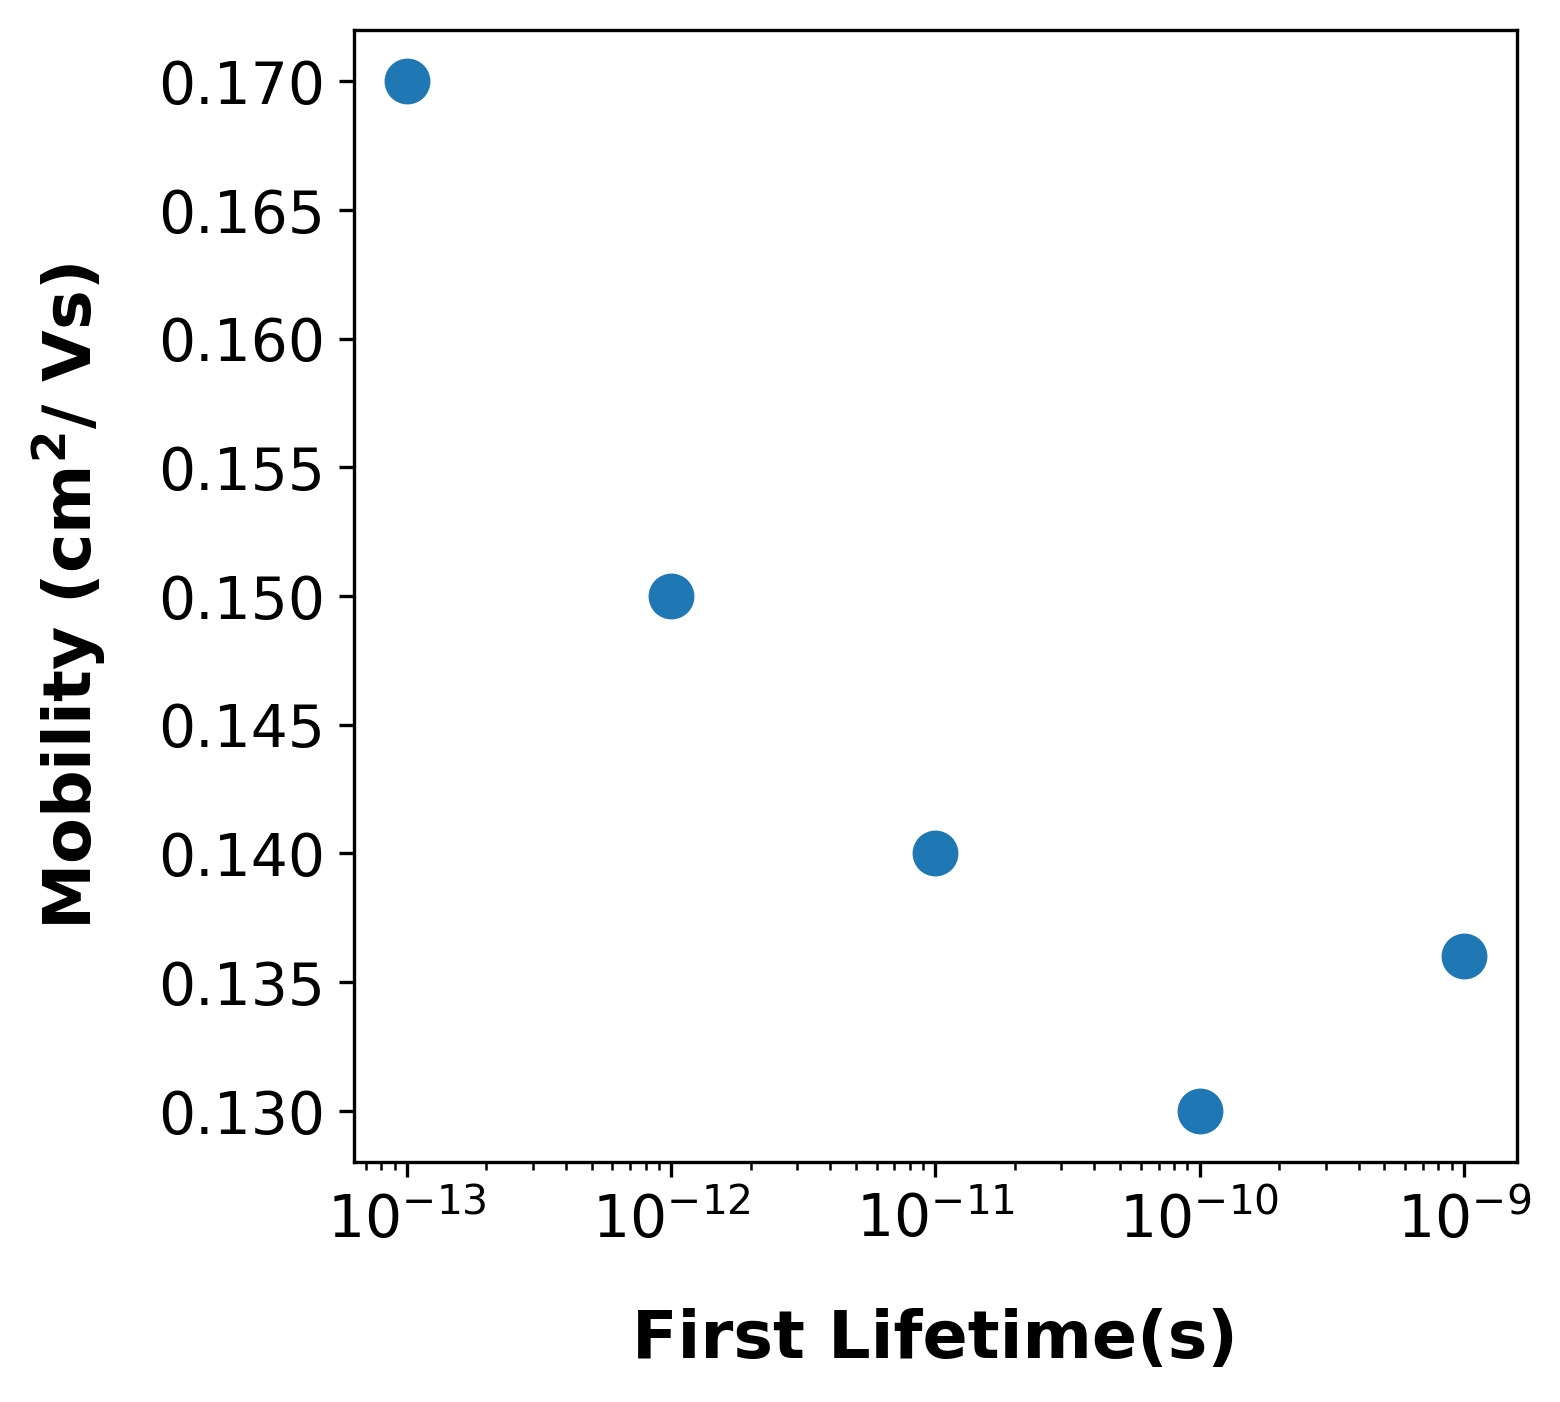
\includegraphics[width=0.8\linewidth]{figures/lifetime.png} 
    \caption{The results of running 5 KMC simulations with the first lifetimes as described in the text. It
    can be seen that below the the ballistic timescale (roughly $10^{-10}$), the resulting mobility is affected}
  \label{lifetime}
\end{figure}

With the slope between MSD at the first lifetime and at the second lifetime proving an estimate of the slope
of the MSD, 6 simulations we run with progressiveily shorter first lifetimes. That is, the second lifetime was
set to $10^{-8}s$ for all 5 simulations and the first lifetime was set to $10^{-9}s$, $10^{-10}s$,
$10^{-11}s$, $10^{-12}s$, and $10^{-13}s$ respectively. The results are plotted in figure
\ref{lifetime}. As expected, as the first lifetime progresses in the ballistic transport timescale, which this work
estimates around $10^{-10}s$, the resulting mobility increases. If the starting lifetime is even shorter the
workflow breaks down becuase as can be seen from the hop rate distribution in figure \ref{TEMP}(D), even at
extreme temperatures, holes need more time that that to hop even once. 

Interestingly, the algorithm seems to be quite robust against choice of lifetimes. As can be seen in the
figure, order of magnitude differences in lifetime choices results in less than 2X difference in the resulting
mobility. This further suggests that going lifetime crazy is a waste of computation.  

\section{ITIC}

To explore the extensibility of the workflow on another benchmark OPV material, using planckton-flow, a 1000
molecule morphology of ITIC was equillibrated over a 10e-7 step MD simulation at room temperature. From the results of the MD
simulation, the last frame of the atomic trajectories is taken to represent an accruate equalibrium geometry
of ITIC. The purpose of this work isnt to justify the efficacy of this type of molecular simulation but it has
been used to affect elsewhere[REFS]. To apply the hopping model to this atomistic morphology requires the
delineation of segments within the morphology upon which charges can delocalize along the within a the HOMO(or in
the case of LUMO for the acceptor). It should be noted that acceptor in this context doesn't refer to
chomophore $j$ as such. Rather, when investigating molecules relevent to electronic devices, acceptors are the
organic analogue of p-type inorganic semiconductors and donors the analogue of the n-type. 
As is well visualized by \cite{Han2019}, the LUMO of ITIC delocalizes along the backbone of the molecule, with
negligible electron density in the side chains. This is visualized in figure \ref{ITIC} using the openly
available visualization tool OVITO \cite{Stukowski2010a}. This makes the the backbone of this kind of small molecule
material the obvious choice. In more polymeric materials like P3HT, the hopping model has received further
justification elsewhere. 

\begin{figure}[]
\centering
\begin{subfigure}{.5\textwidth}
    \textbf{(A)}
    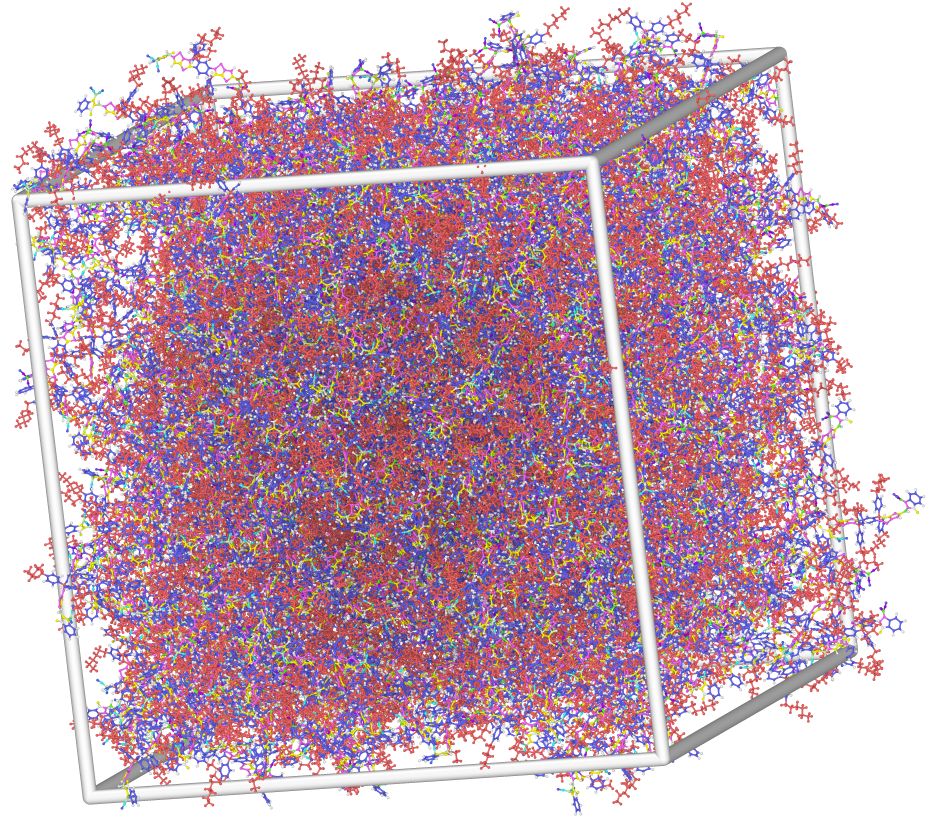
\includegraphics[width=\textwidth]{figures/ITIC-blackedout-unwrapped-allatom.png}
\end{subfigure}%
\begin{subfigure}{.5\textwidth}
    \textbf{(B)}
    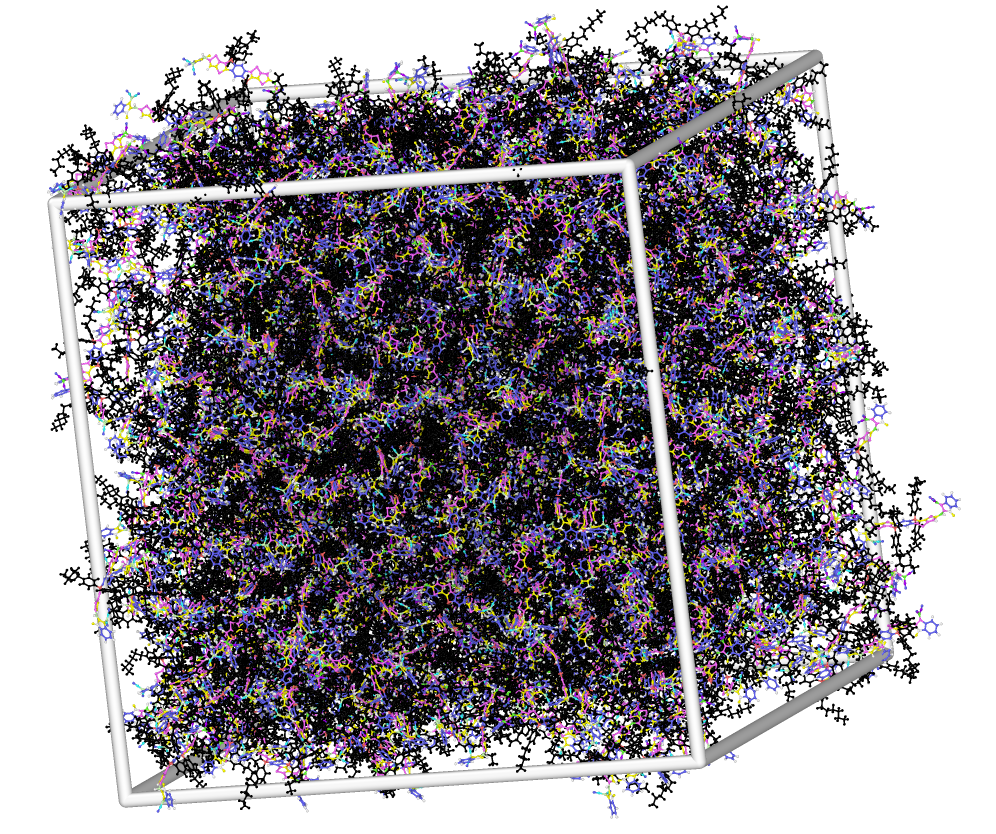
\includegraphics[width=\textwidth]{figures/ITIC-blackedout-unwrapped.png}
\end{subfigure}
    \caption[short]{1000 molecule ITIC morphology. Figure (B) shows segments known to participate in frontier
    molecular orbitals in color and side chains in black.}
\label{ITIC}
\end{figure}



The the reported
experimental electron mobility of ITIC varies depending on how it was processed and how it was measured. Time-of-flight electron mobilities on the order of $10^{-4}$ \cite{Mica2018} and field effect mobilities on the order of
$10^{-2}$ \cite{Park2018} have been reported. 

\section{Improvements}

In this work, we ignore dynamic disorder by doing calculations on snapshots from equillibrium MD simulations.
Others have had success intruducing dynamic disorder via nudging the QQC calculated TI value at every
iteration of the KMC algorithm by a number drawn randomly from a Gaussian Distribtion \cite{Gali2017}.

Dynamic disorder does effect charge mobility (CT in high mobility conjugated polymers) with every pico second
may have a 10-20\% fluxuation in TI. Need to find the paper but using the dynamic dimer methor for TI calc
could be a way to introduce dynamic disorder. Or it could be done as mentioned before in another paper where
they use two different methods one with a guassians fluxuation and sime ohther fancy method. 

In our kmc algorithm we could incorperate the rates of other events like recombination.

The computational bottle neck of simulation charge mobility is also the most theoretically challenging.
Estimating the TI for each pair of chromophores. A future improvement to MorphCT will be accelerating this step
with Machine learning techniques. Musil et al. have shown that ML could produce a 90 \% decrease in
computational effort \cite{Musil2018}

Something to do is allow morphct as to figure out what to do with donor accpeter mixtures. It would be pretty
easy to run asyncronously on the donor/acceptor materials and compare. this could be a measure of morphology.
If you run pure donor and pure acceptor and you got mobities, if on of those drops in the mixed morph more
that the other you probably dont have a nice domain for BHJ.

I hope one day a submission to a quantum computer could solve with extreme precicission the shrodinger
equation for an entire morphology. Quantum algorithms are most advanced in this space and we await the race
to large qubit computers. 

I havent looked into it but I think reorganization energry should scale in out algorythm with crystallinity
iasfaras we can measure crystallinity. the external reorganization energy of the material ,at least for p3ht
was 200, and thats the lions share of overall reorganization energy which we have all ready shown to
monitonically scale with the calculated mobilioty in this algorith. But external reorganization energy is
related to the distortion of the surrounding medium. if the surrounding medium is shaped like a net if will
certainly distort less than a disordered medium. Maybe this all ready talked about but energy does scale with
molucaler size and rigidity \cite{McMahon2010a}

%%% Local Variables: 
%%% mode: latex
%%% TeX-master: "BSUmain"
%%% End: 
